\RequirePackage{luatex85}
\documentclass[varwidth]{standalone}

% Preamble
\usepackage{booktabs}
\usepackage{graphicx}
\usepackage{subcaption}
\captionsetup{justification=raggedright,singlelinecheck=false}
\renewcommand{\familydefault}{\sfdefault}
\renewcommand\thesubfigure{(\alph{subfigure})}
\usepackage{xcolor}
\renewcommand\fbox{\fcolorbox{white}{white}}
\usepackage{todonotes}

\begin{document}

\begin{figure}
    \centering
    \begin{subfigure}[t]{0.49\textwidth}
        \setcounter{subfigure}{0}
        \caption{}
        \fbox{%
        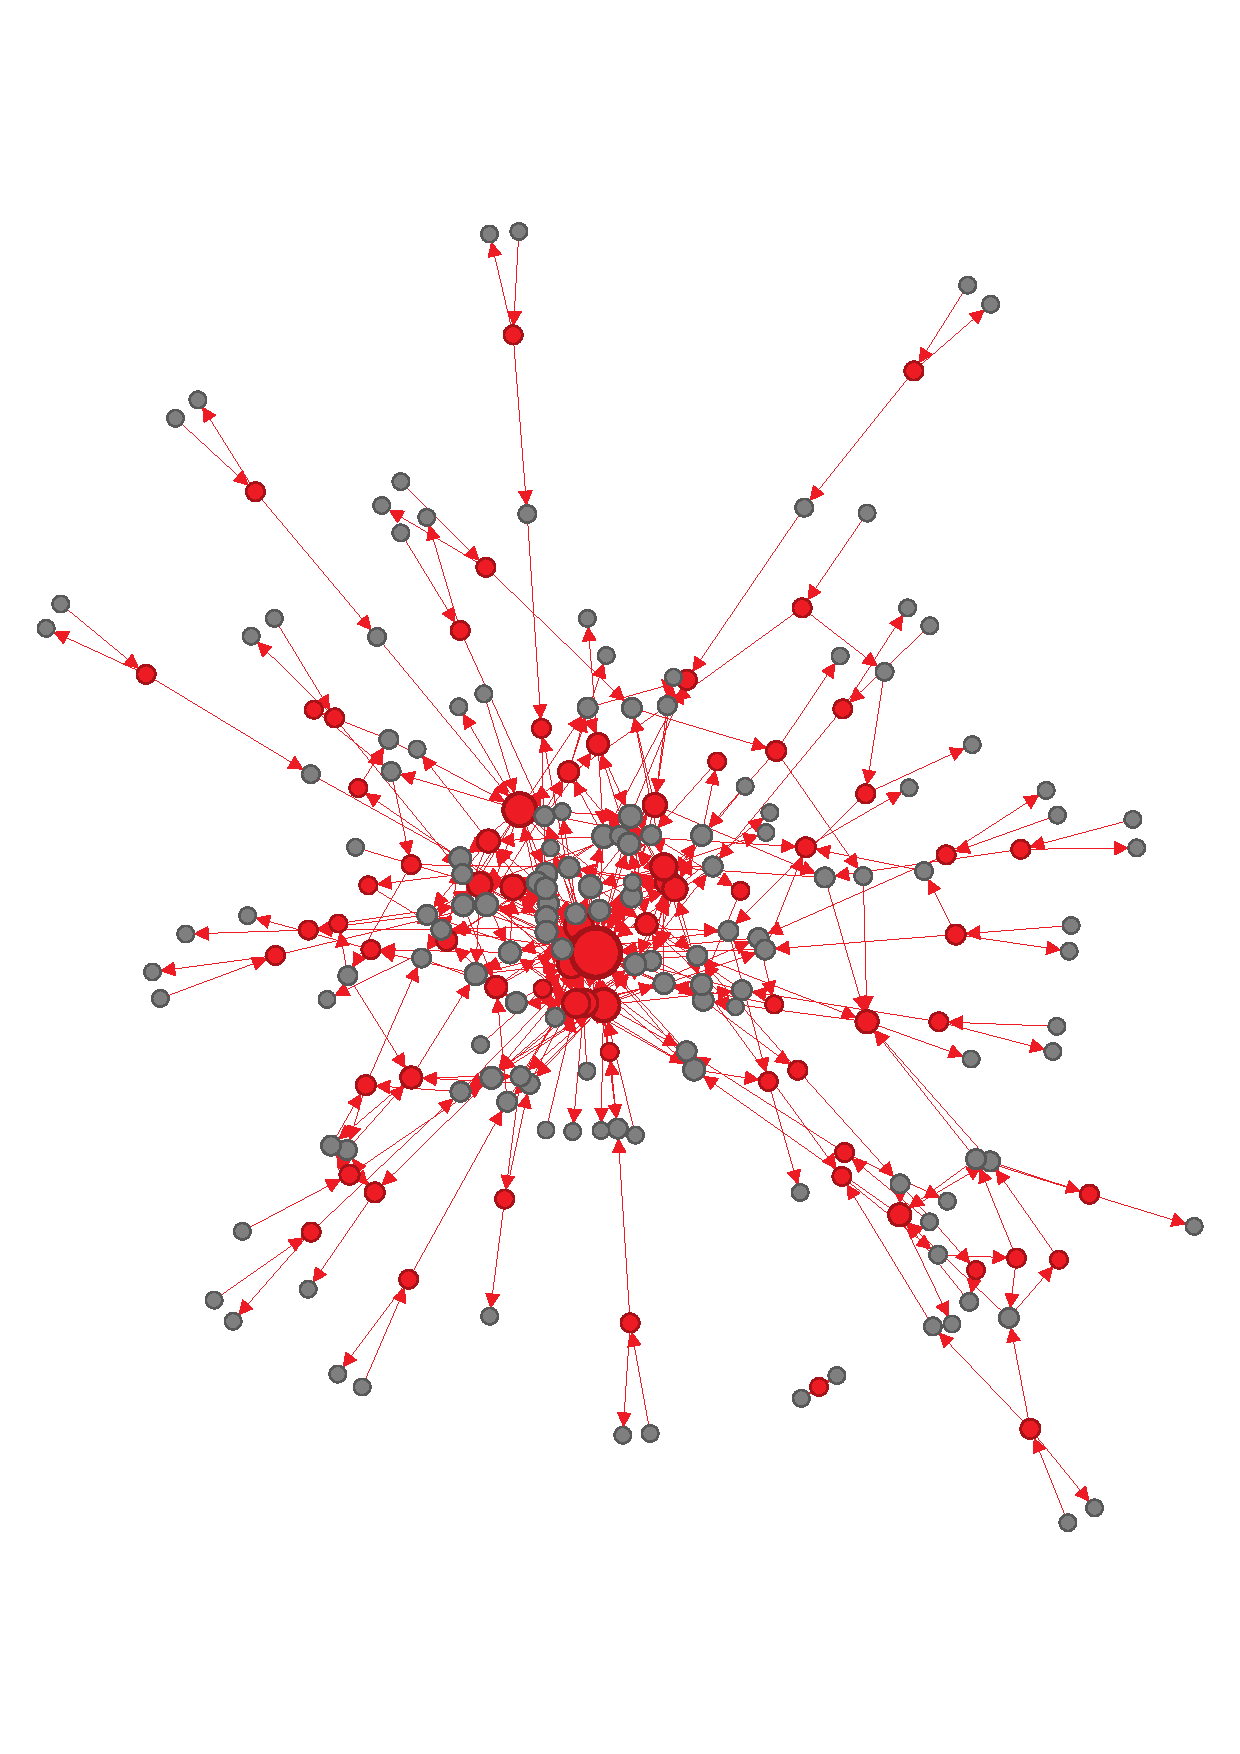
\includegraphics[width=\textwidth, trim={0 3.5cm 0 3.5cm}, clip]{from-gephi/catalyst-network-e_coli_core-bipartite.pdf}
        }
    \end{subfigure}
    \begin{subfigure}[t]{0.49\textwidth}
        \setcounter{subfigure}{1}
        \caption{}
        \fbox{%
        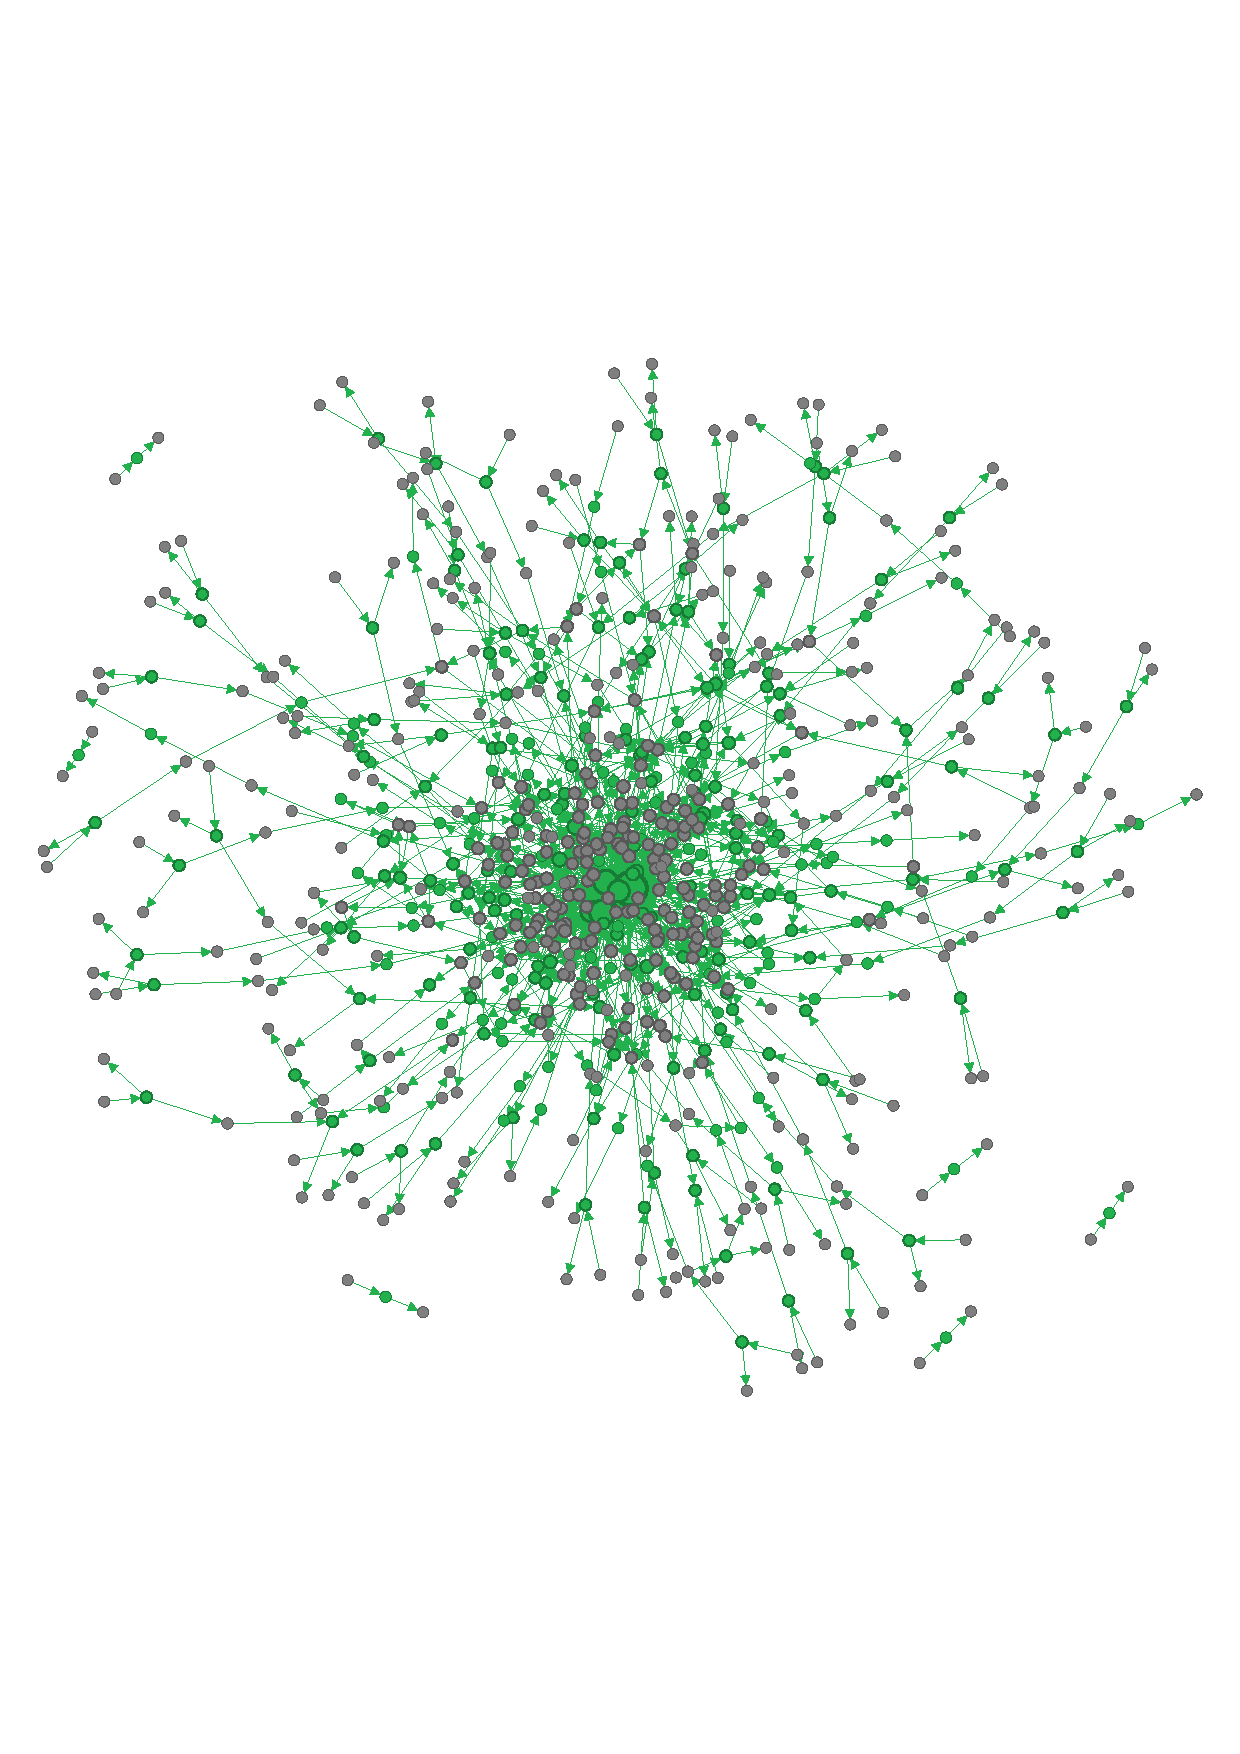
\includegraphics[width=\textwidth, trim={0 3.5cm 0 3.5cm}, clip]{from-gephi/catalyst-network-iAB_RBC_283-bipartite.pdf}\\
        }
    \end{subfigure}
    \begin{subfigure}[t]{0.49\textwidth}
        \setcounter{subfigure}{2}
        \vspace*{-3.0ex}
        \caption{}
        \fbox{%
        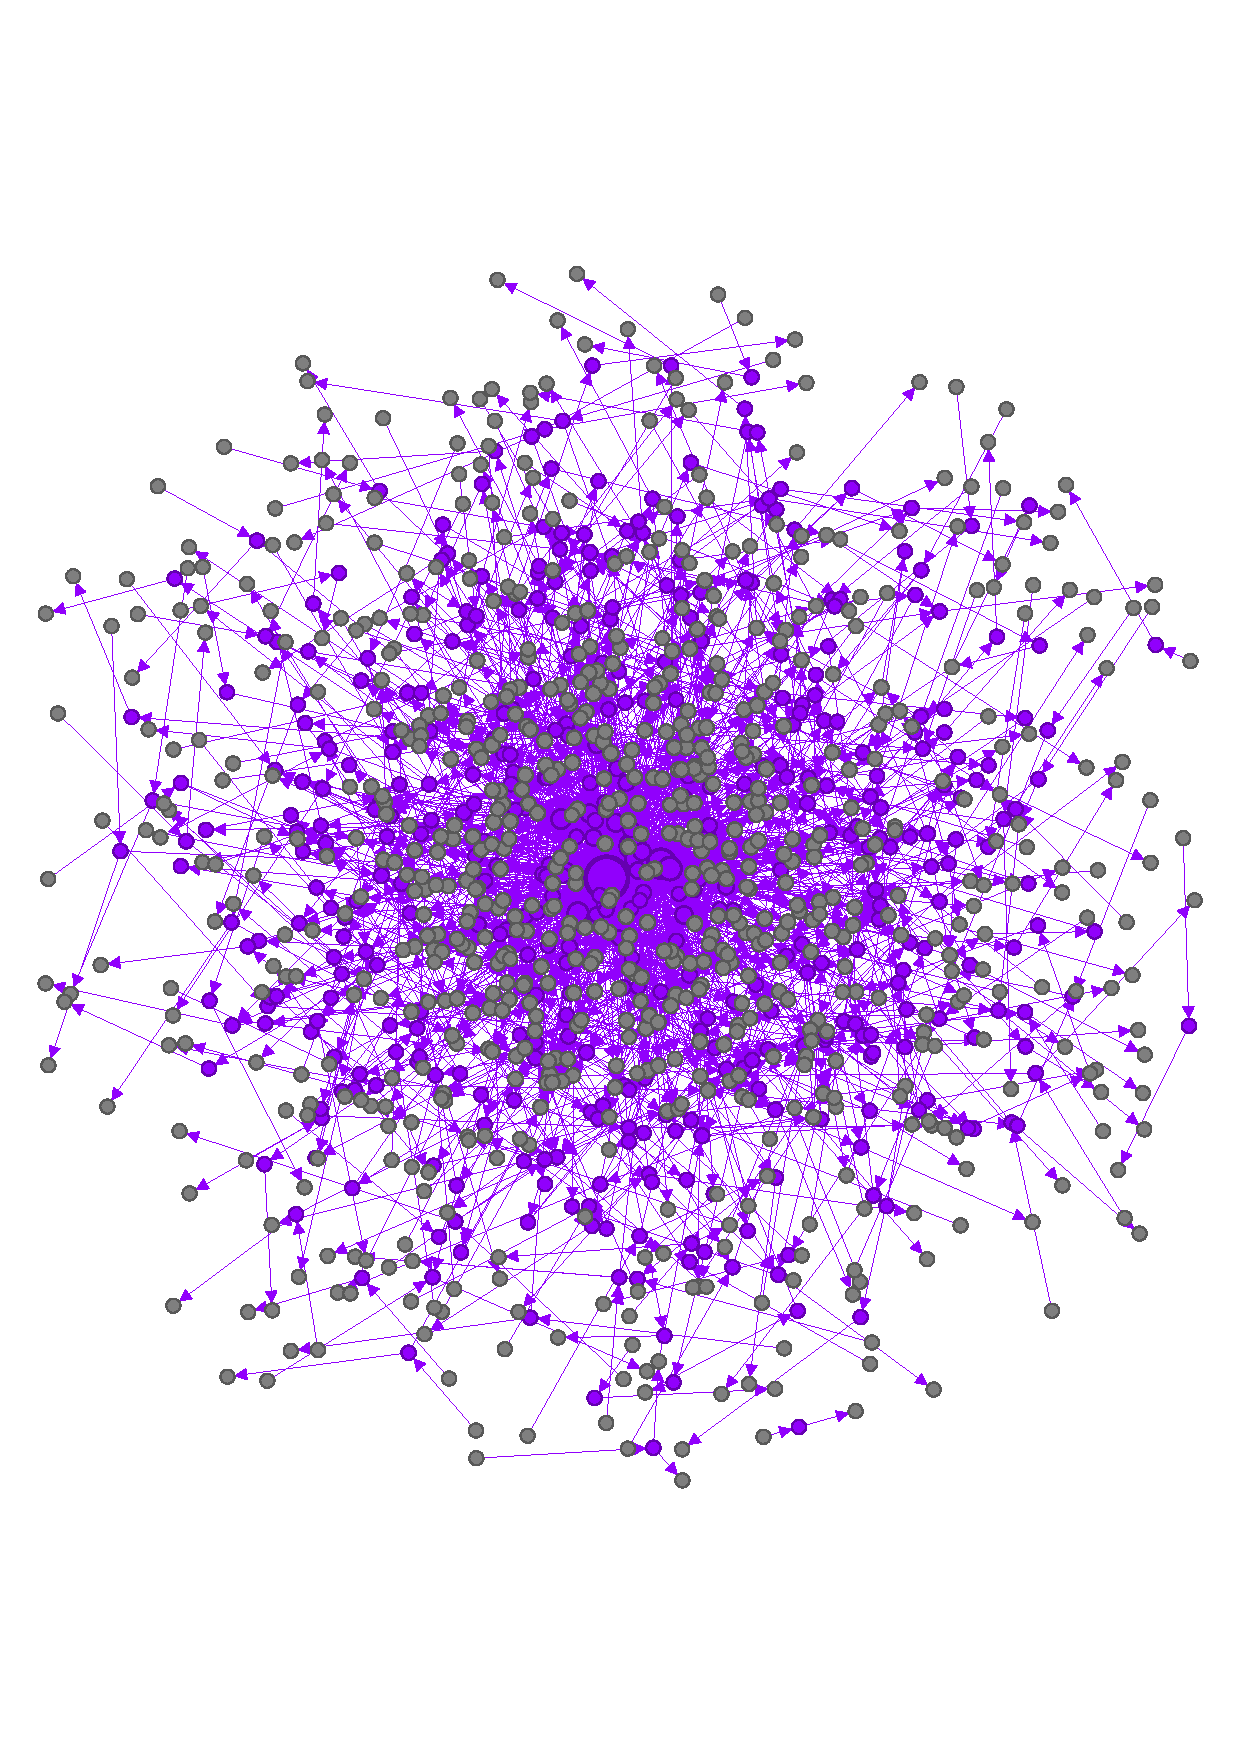
\includegraphics[width=\textwidth, trim={0 4.0cm 0 4.0cm}, clip]{from-gephi/catalyst-network-iIT341-bipartite.pdf}
        }
    \end{subfigure}
    \begin{subfigure}[t]{0.49\textwidth}
        \setcounter{subfigure}{3}
        \vspace*{-3.0ex}
        \caption{}
        \fbox{%
        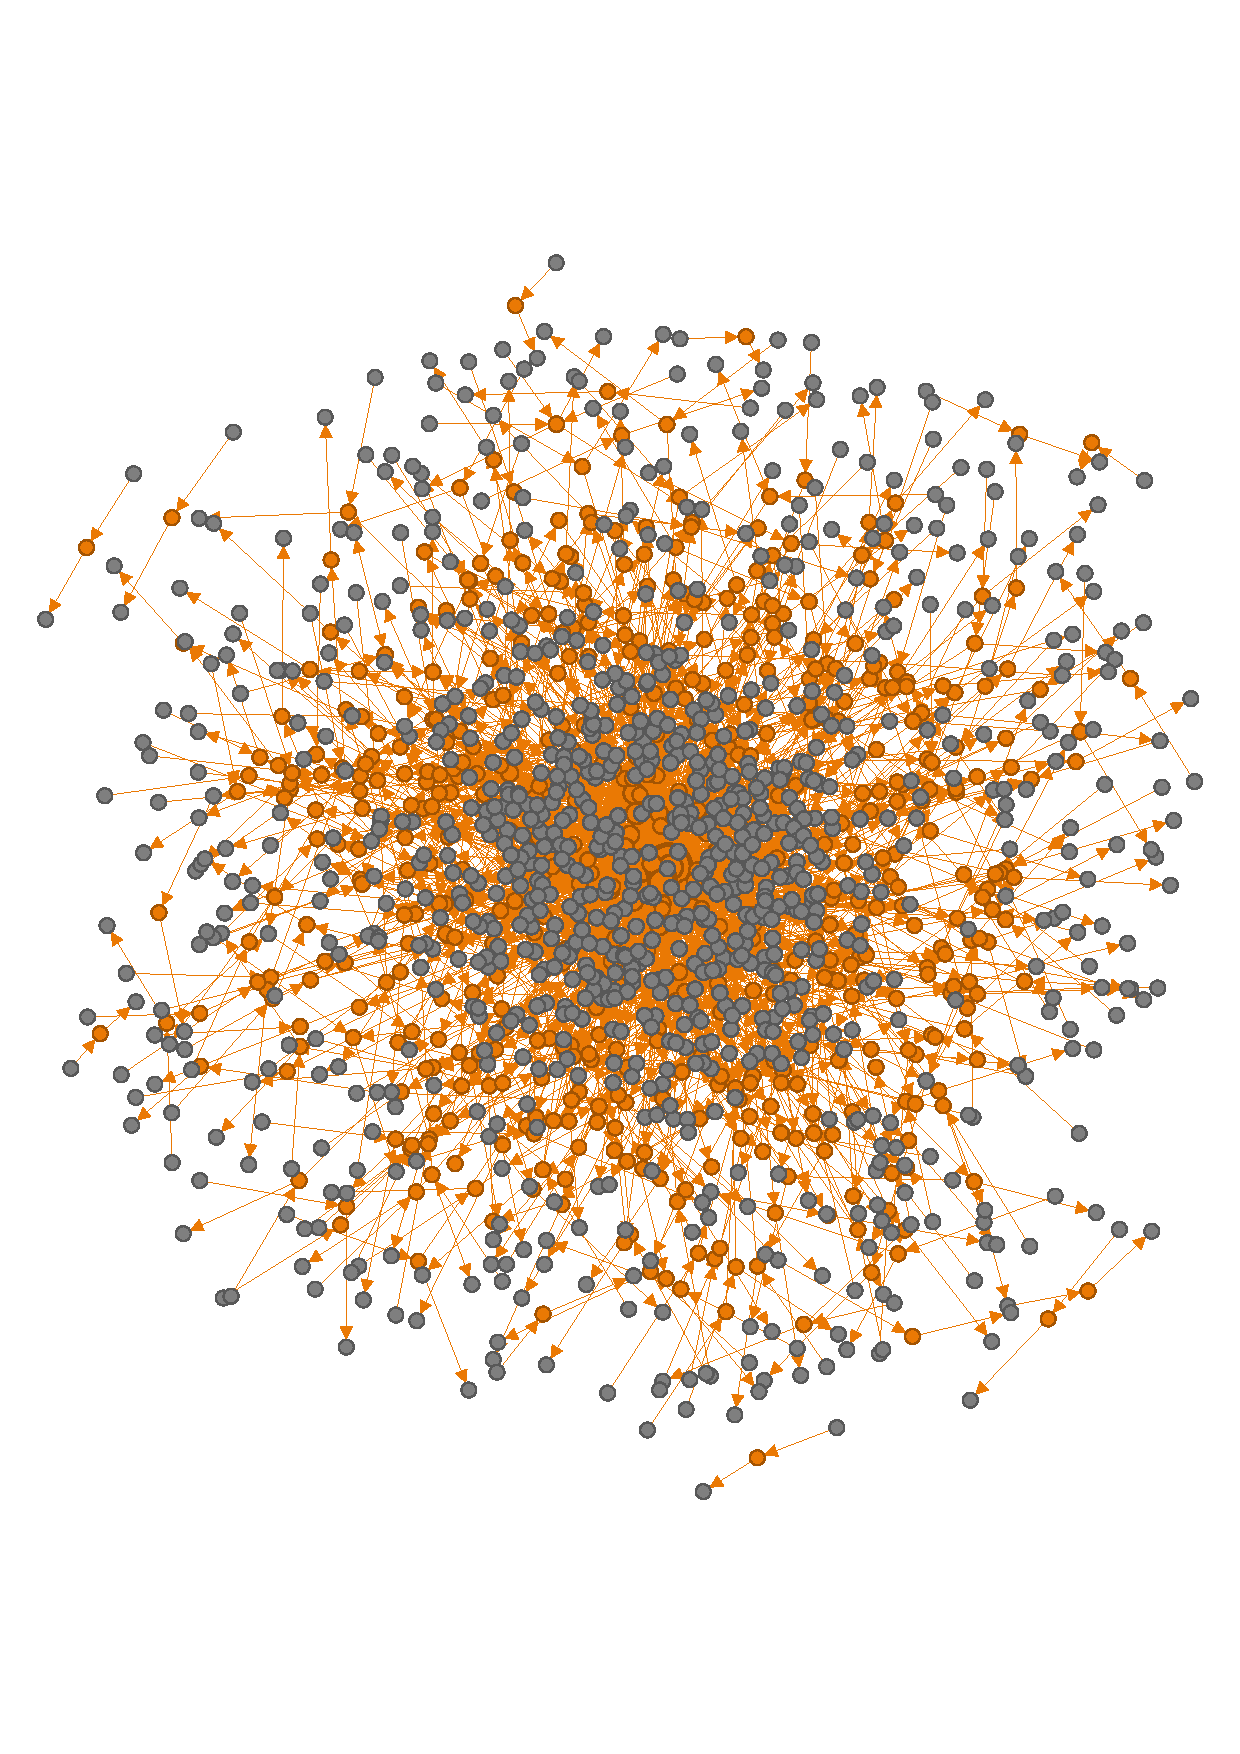
\includegraphics[width=\textwidth, trim={0 4cm 0 4cm}, clip]{from-gephi/catalyst-network-iSB619-bipartite.pdf}
        }
    \end{subfigure}
    \begin{subfigure}[t]{0.49\textwidth}
        \setcounter{subfigure}{4}
        \vspace*{-5.0ex}
        \caption{}
        \fbox{%
        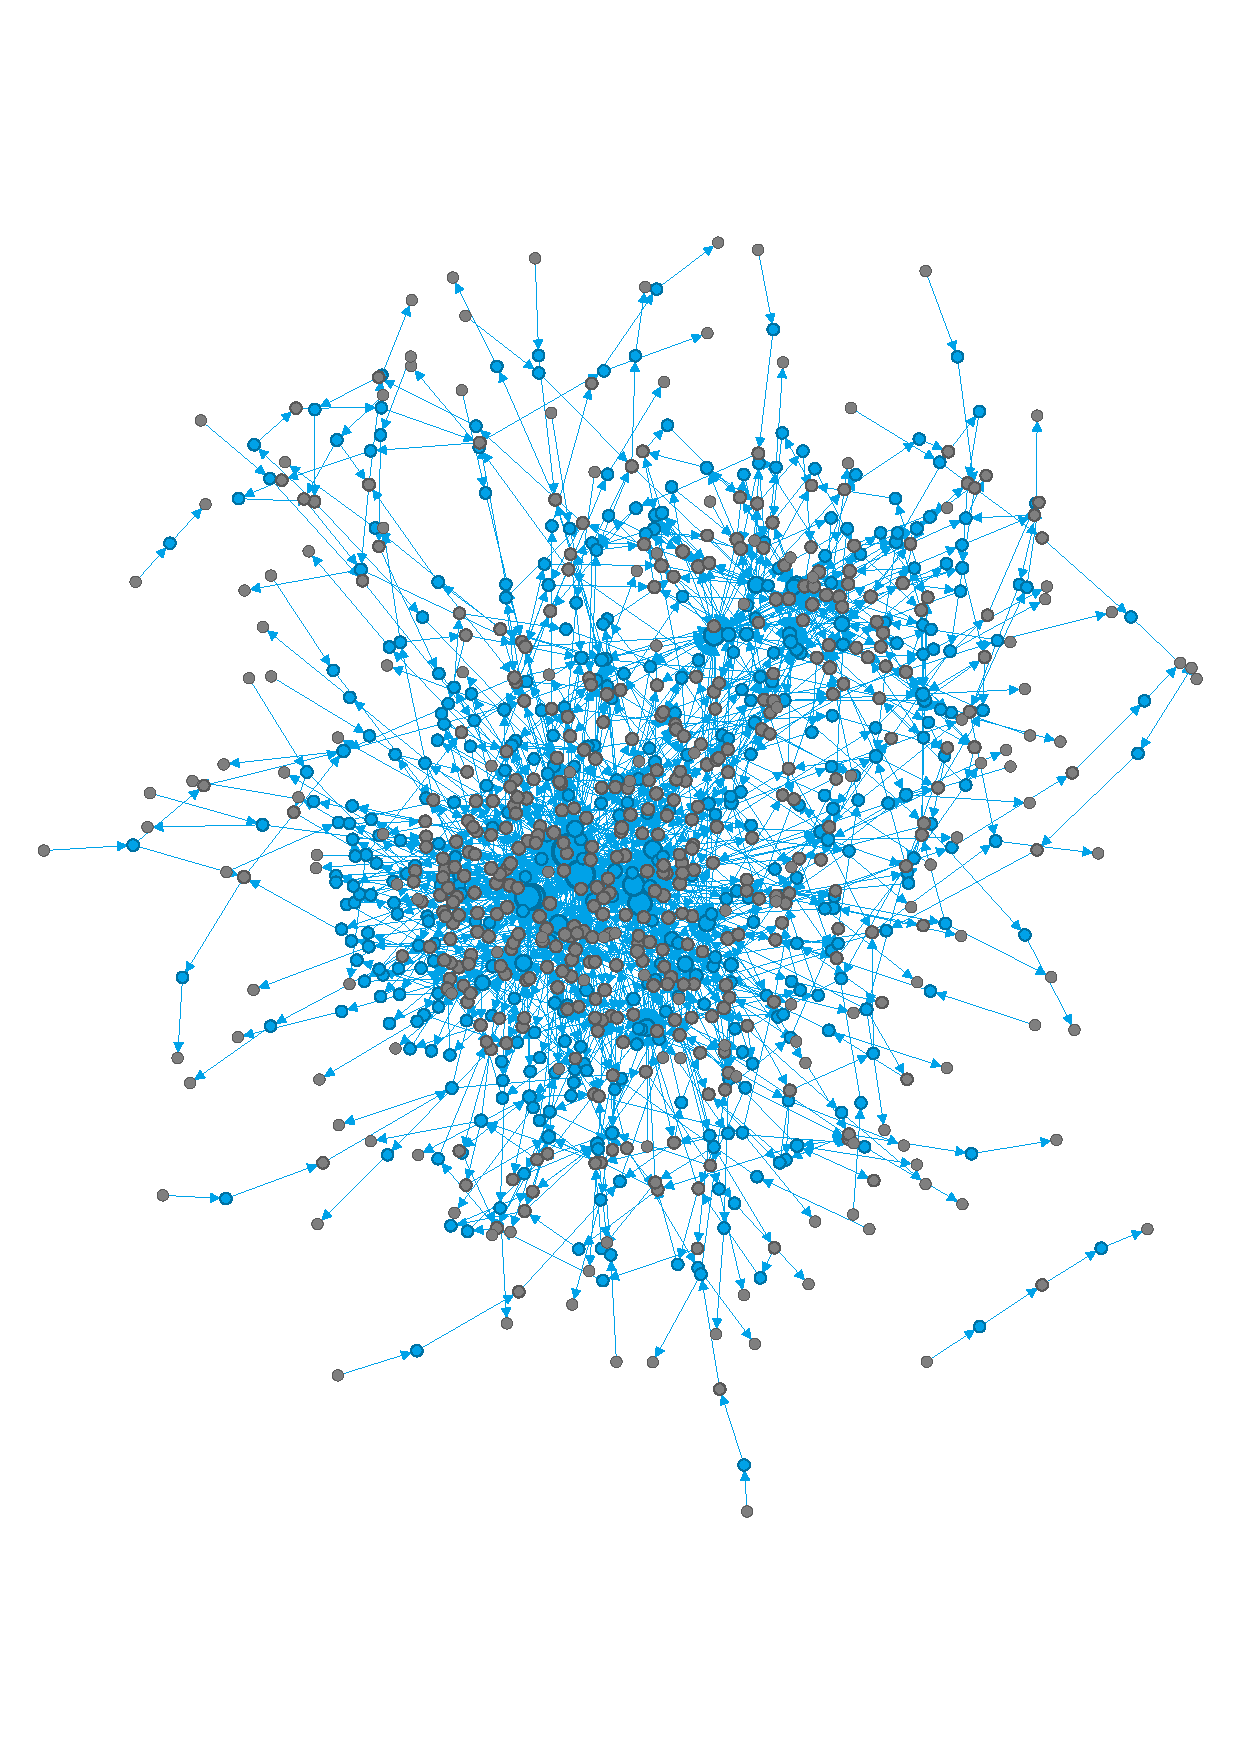
\includegraphics[width=\textwidth, trim={0 4cm 0cm 4cm}, clip]{from-gephi/catalyst-network-hepg2-bipartite.pdf}
        }
    \end{subfigure}
    \begin{subfigure}[t]{0.49\textwidth}
        \fbox{}
    \end{subfigure}
    %\caption{%
        %Visualization of the five GEMs as bipartite graphs with metabolites and reactions denoted as coloured and grey nodes. (a) E. coli core. (b) iAB RBC 283. (c) iIT341. (d) iSB619. (e) HepG2.
    %}
\end{figure}
  
\end{document}


